\section{Appendix}\label{sec:appendix}

\subsection{Example Function Help-file}\label{fig:ex-help}

\begin{figure} [!htb]
    \centering
    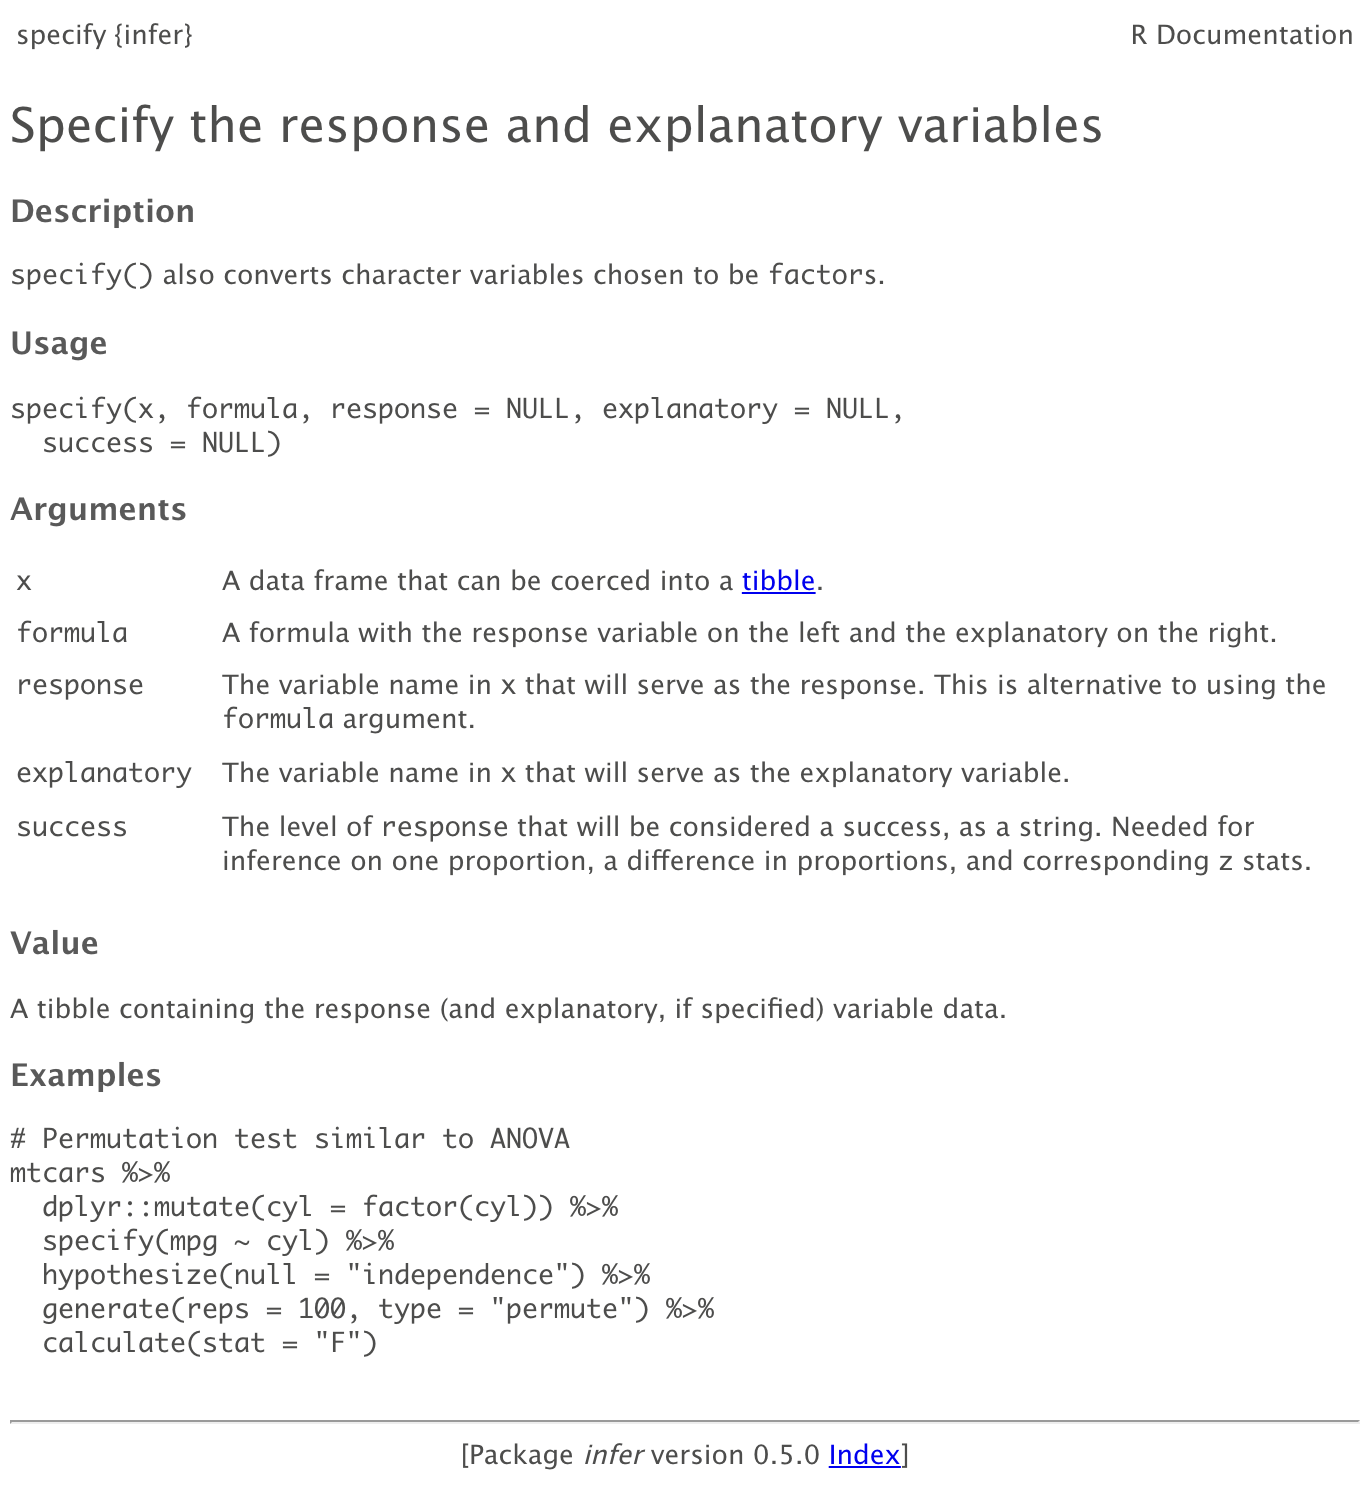
\includegraphics[width=.9\linewidth]{figures/ex_help.png}
    \caption*{A typical example function help-file, describing the \textit{specify} function from version 0.5.0 of the \textit{infer} R package. Function help-files often contain a basic description of the function, the syntax for executing the function, the format of user inputs and outputs, and, often, a practical example demonstrating usage.}
\end{figure}

\clearpage

\subsection{Semi-Structured Interview Protocol}\label{sec:interview}

\begin{itemize}
    \item What makes documentation effective?
    \item What have conversations with (other) tidyverse developers about documentation practices looked like? 
    \item Were there disagreements about any practices?
    \item Is documentation written differently within the tidyverse versus outside of it? (How so? Why might that be?)
    \item What are the consequences of ineffective documentation?
    \item Do gender minorities interact with documentation differently? How so?
    \item How do the demographics of the tidyverse community compare to those in the greater R community?
    \item How do the demographics of the tidyverse community differ from those in other user communities you've been a part of?
    \item I’ve found so far that tidyverse packages are more likely to have package-level help-files, and that function-level help-files from the tidyverse have a greater character count, more examples, more comments per example, and more references to related functions than help-files from non-Tidy libraries. Is this surprising? (What mechanisms might be driving these differences?)
\end{itemize}
